\documentclass[11pt]{article}

% ---------------------------------------------------------------------------
%  Coproduct of generators, product of concepts.
%  A standalone research note: why an ADDITIVE (disjoint-union) closure code
%  represents a MULTIPLICATIVE (direct-product) concept lattice.
%  Compiles with pdflatex + bibtex on Overleaf. Self-contained (all TikZ).
% ---------------------------------------------------------------------------

\usepackage[a4paper,margin=2.6cm]{geometry}
\usepackage{lmodern}   % scalable Type1 fonts (needed for microtype expansion)
\usepackage[T1]{fontenc}
\usepackage{amsmath,amssymb,amsthm}
\usepackage{booktabs}
\usepackage{xcolor}
\usepackage{tikz}
\usepackage{pgfplots}
\pgfplotsset{compat=1.17}
\usetikzlibrary{positioning,arrows.meta,fit,backgrounds,calc,shapes.geometric}
\usepackage[hidelinks]{hyperref}
\usepackage{microtype}

% ---- colours (shared with concept-dag-note.tex) -----------------------
\definecolor{cAttr}{RGB}{70,130,180}    % attributes (steel blue)
\definecolor{cConc}{RGB}{200,120,40}     % concepts (amber)
\definecolor{cGood}{RGB}{40,140,80}      % green
\definecolor{cBad}{RGB}{190,60,60}       % red
\definecolor{cFacA}{RGB}{70,130,180}     % factor A
\definecolor{cFacB}{RGB}{150,80,160}     % factor B (purple)
\definecolor{cGrid}{RGB}{210,210,210}

% ---- theorem environments ---------------------------------------------
\theoremstyle{definition}
\newtheorem{definition}{Definition}
\theoremstyle{plain}
\newtheorem{lemma}{Lemma}
\newtheorem{theorem}{Theorem}
\newtheorem{corollary}{Corollary}
\theoremstyle{remark}
\newtheorem{remark}{Remark}

% ---- handy macros ------------------------------------------------------
\newcommand{\cl}{\operatorname{cl}}       % closure of a node
\newcommand{\Dcode}{\mathsf{D}}            % decoder
\newcommand{\Lgen}{\mathcal{L}}            % generated lattice
\newcommand{\Gcoprod}{\sqcup}             % coproduct / disjoint union
\newcommand{\attrs}{M}
\newcommand{\bits}{\ \text{bits}}

\title{\bf Coproduct of Generators, Product of Concepts\\[3pt]
\large Why an \emph{additive} closure code represents a \emph{multiplicative}
concept lattice --- a lattice-theoretic statement of the factorial-code
compression, with a proof and an experiment}
\author{Peter F\"oldi\'ak}
\date{\today}

\begin{document}
\maketitle

\begin{abstract}
\noindent
Formal Concept Analysis converts a table of yes/no facts into a
\emph{concept lattice}. When the attributes split into two independent groups
--- ``size'' and ``colour,'' say --- the lattice of the combined data is (up to
which combinations actually occur) the \emph{direct product} of the two
per-group lattices: one node for every pair, so the node count \emph{multiplies}.
That is the blow-up that makes people reach for a factorised representation and
ask whether one should learn the factors directly rather than build the product
and try to factor it afterwards. This note isolates the clean fact underneath
that worry, independently of any particular learning algorithm. We model a
concept system as a set of \emph{generators} (a directed acyclic graph of
concepts over attribute sinks) decoded by \emph{downward closure}: an object
switches on an antichain of generators and inherits the union of the attributes
below them. We prove that the \emph{coproduct} (disjoint union) of two such
generators over disjoint attribute alphabets generates exactly the \emph{direct
product} of the two lattices they generate individually. The generator combines
\emph{additively} ($m+n$ nodes) while the represented concept lattice combines
\emph{multiplicatively} ($m\cdot n$ nodes). We give the theorem in a decoder-agnostic
form (it is really a statement about \emph{separable decoders on disjoint output
alphabets}, not about DAGs), work a small example by hand, connect it to
Barlow's factorial codes and to the classical FCA facts about apposition and
subdirect products, and confirm it with an experiment in which a
description-length learner, handed two independent planted hierarchies, returns
the two factors and \emph{zero} cross-factor concepts, representing all their
combinations in the object codes. We close with the boundary conditions worth
remembering --- disjoint alphabets, statistical independence, and realisability
--- and with why ``learn the neural code'' and ``learn the DAG'' turn out not to
be a dichotomy.
\end{abstract}

\tableofcontents

% =======================================================================
\section{The phenomenon this note is about}
% =======================================================================

Two independent axes of variation, each with its own little hierarchy, produce a
combined concept system whose size is the \emph{product} of the two. If
``size'' has three meaningful values (small $\subset$ medium $\subset$ large as
attribute sets) and ``colour'' likewise (red, warm, any), then ``small red,''
``medium warm,'' ``large any'' and every other pairing is a legitimate closed
concept of the combined data. Formal Concept Analysis (FCA)~\cite{ganter1999}
will faithfully build all $3\times 3 = 9$ of them, and with $k$ independent
binary axes it will build $2^{k}$. The lattice is correct; it is just
\emph{exponentially larger than the description of the world it came from}. The
world was two (or $k$) small independent parts.

The instinct this provokes --- and it is the right instinct --- is that the
meaningful object is not the big product lattice but a \emph{factorisation} of
it: keep the parts, and reconstruct any combination on demand. One could
build the product and then try to factor it (hard: it is the subdirect
decomposition problem, of which more in \S\ref{sec:buys}), or one could
\emph{generate the factors in the first place} and never form the product at all.

This note is about the second option, and about one fact that makes it work
cleanly. Informally:

\begin{quote}
\emph{If you store the two factors side by side (an additive combination of
generators) and decode by downward closure, the set of concepts you can
represent is already the full product --- you get the multiplicative lattice for
the additive price, and you never build the product explicitly.}
\end{quote}

Everything below makes ``store side by side,'' ``decode by closure,'' ``the
lattice you can represent,'' and ``the full product'' precise, proves the
identity between them, and marks exactly where it stops holding. The result is
stated so that it stands on its own as a fact about closure codes and factorial
representations; the description-length learner that motivated it appears only in
\S\ref{sec:experiment} as a confirmation and in \S\ref{sec:project} as the
application.

% =======================================================================
\section{Generators and the lattice they generate}
\label{sec:generators}
% =======================================================================

Fix a finite set of \emph{attributes} $\attrs$ (the observable features; in FCA
terms, the columns of a context). We describe a concept system not by listing its
concepts but by a small \emph{generator} that produces them.

\begin{definition}[Closure DAG]
A \emph{closure DAG} $G$ over $\attrs$ is a finite directed acyclic graph whose
sinks are the attributes $\attrs$ and whose remaining nodes are \emph{concepts}.
For a node $k$, its \emph{closure} $\cl_G(k)\subseteq\attrs$ is the set of
attributes reachable from $k$ (the attributes ``below'' it). Edges point from a
concept to its children (concepts or attributes).
\end{definition}

An object does not name a concept lattice; it switches on a few generators and
inherits everything below them.

\begin{definition}[Antichain code and its decoding]
A \emph{code} is an antichain $S$ of nodes of $G$ (no node of $S$ reachable from
another). It \emph{decodes} to the attribute set
\[
  \Dcode_G(S)\;=\;\bigcup_{k\in S}\cl_G(k)\;\subseteq\;\attrs .
\]
The \emph{generated family} is $\Lgen(G)=\{\Dcode_G(S): S \text{ an antichain of } G\}$.
\end{definition}

The antichain restriction loses nothing at the level of \emph{what can be
represented}: closure is monotone along reachability (if $u$ is reachable from
$v$ then $\cl_G(u)\subseteq\cl_G(v)$), so in any set of nodes the topmost ones
already contribute every attribute the lower ones would. Hence
$\Lgen(G)=\bigl\{\bigcup_{k\in T}\cl_G(k): T\subseteq \text{nodes}\bigr\}$, the
family of attribute sets obtainable as \emph{any} union of node-closures
(the antichain is merely the non-redundant way to name each such set).

\begin{lemma}[$\Lgen(G)$ is a lattice]
\label{lem:lattice}
$\Lgen(G)$, ordered by $\subseteq$, is a finite lattice. Join is union
($A\vee B=A\cup B$, which lies in $\Lgen(G)$ because the family is closed under
union); meet is $A\wedge B=\bigcup\{C\in\Lgen(G):C\subseteq A\cap B\}$, the
largest member below both. Its bottom is $\varnothing$ (the empty union) and its
top is $\bigcup_k \cl_G(k)$.
\end{lemma}

\begin{proof}
$\Lgen(G)$ is closed under $\cup$ by construction (a union of two node-unions is a
node-union) and contains $\varnothing$. A finite $\cup$-closed family containing
its own empty join is a lattice: the displayed meet is a member (again a union of
members), is $\subseteq A\cap B$, and dominates every member below both, so it is
the greatest lower bound.
\end{proof}

$\Lgen(G)$ is the concept lattice \emph{our generator commits to}: exactly the
attribute sets some object can be predicted to have. It need not be the full FCA
lattice of any particular data set --- that depends on the data --- but it is the
right object for asking ``what can this generator represent?''.

\begin{figure}[h]
\centering
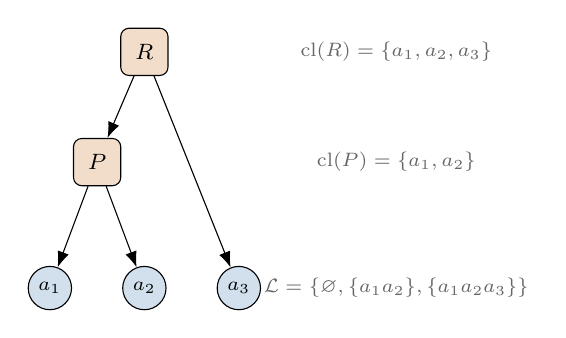
\begin{tikzpicture}[
   node distance=6mm,
   attr/.style={draw,circle,fill=cAttr!25,minimum size=5.5mm,inner sep=0pt,font=\scriptsize},
   con/.style={draw,rounded corners=3pt,fill=cConc!25,minimum size=6mm,inner sep=2.5pt,font=\footnotesize\bfseries}]
  \foreach \i in {1,2,3}
    \node[attr] (a\i) at (\i*1.2,0) {$a_{\i}$};
  \node[con] (P) at (1.8,1.6) {$P$};
  \node[con] (R) at (2.4,3.0) {$R$};
  \draw[-{Latex[length=2mm]}] (P)--(a1); \draw[-{Latex[length=2mm]}] (P)--(a2);
  \draw[-{Latex[length=2mm]}] (R)--(P);  \draw[-{Latex[length=2mm]}] (R)--(a3);
  \node[font=\scriptsize,align=left,text=black!60] at (5.6,3.0)
     {$\cl(R)=\{a_1,a_2,a_3\}$};
  \node[font=\scriptsize,align=left,text=black!60] at (5.6,1.6)
     {$\cl(P)=\{a_1,a_2\}$};
  \node[font=\scriptsize,align=left,text=black!60] at (5.6,0.0)
     {$\Lgen=\{\varnothing,\{a_1a_2\},\{a_1a_2a_3\}\}$};
\end{tikzpicture}
\caption{A one-factor closure DAG and the $3$-element chain it generates. The two
concept nodes $P\subset R$ (with $R$ adding $a_3$) generate the chain
$\varnothing\subset\{a_1a_2\}\subset\{a_1a_2a_3\}$. Two generators, three
concepts.}
\label{fig:onefactor}
\end{figure}

% =======================================================================
\section{Two ways to combine two concept systems}
% =======================================================================

Let $G_1$ over $\attrs_1$ and $G_2$ over $\attrs_2$ be two closure DAGs. There
are two very different things one might mean by ``putting them together.''

\begin{definition}[Direct product of lattices]
The \emph{direct product} $\Lgen(G_1)\times\Lgen(G_2)$ has as elements all ordered
pairs $(A,B)$ with $A\in\Lgen(G_1)$, $B\in\Lgen(G_2)$, ordered
\emph{componentwise}: $(A,B)\le(A',B')$ iff $A\subseteq A'$ and $B\subseteq B'$.
Meet and join are componentwise. Its size is
$|\Lgen(G_1)|\cdot|\Lgen(G_2)|$ --- \emph{multiplicative}.
\end{definition}

\begin{definition}[Coproduct of generators]
Assume $\attrs_1\cap\attrs_2=\varnothing$. The \emph{coproduct}
$G_1\Gcoprod G_2$ is the disjoint union of the two DAGs: node set the disjoint
union of the two node sets, edges exactly those of $G_1$ and of $G_2$ (\emph{no
edges between the parts}), attribute set $\attrs_1\sqcup\attrs_2$. Its size
(nodes, edges) is $|G_1|+|G_2|$ --- \emph{additive}.
\end{definition}

The direct product is an operation on the \emph{generated lattices} and it is the
expensive, ``unfolded'' object. The coproduct is an operation on the
\emph{generators} and it is the cheap, ``folded'' object: you literally lay the
two graphs side by side and change nothing. The content of this note is that,
under closure decoding, the cheap folded thing generates the expensive unfolded
thing.

\begin{figure}[h]
\centering
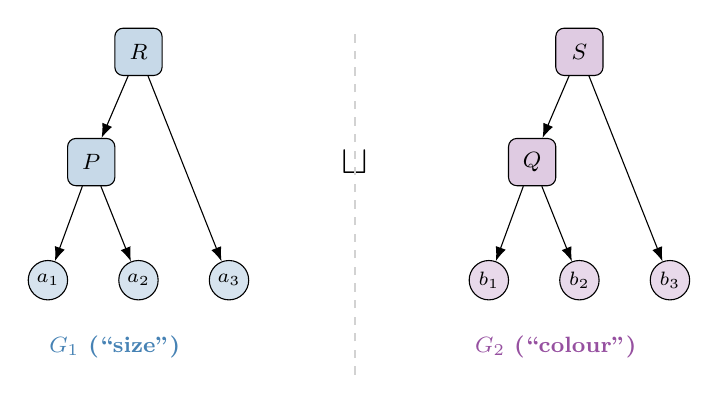
\begin{tikzpicture}[
   node distance=5mm,
   attr/.style={draw,circle,minimum size=5mm,inner sep=0pt,font=\scriptsize},
   con/.style={draw,rounded corners=3pt,minimum size=6mm,inner sep=2pt,font=\footnotesize\bfseries}]
  % Factor A
  \begin{scope}
    \foreach \i in {1,2,3}
      \node[attr,fill=cFacA!22] (a\i) at (\i*1.15,0) {$a_{\i}$};
    \node[con,fill=cFacA!30] (P) at (1.7,1.5) {$P$};
    \node[con,fill=cFacA!30] (R) at (2.3,2.9) {$R$};
    \draw[-{Latex[length=1.8mm]}] (P)--(a1); \draw[-{Latex[length=1.8mm]}] (P)--(a2);
    \draw[-{Latex[length=1.8mm]}] (R)--(P);  \draw[-{Latex[length=1.8mm]}] (R)--(a3);
    \node[font=\footnotesize\bfseries,text=cFacA] at (2.0,-0.85) {$G_1$ (``size'')};
  \end{scope}
  % Factor B
  \begin{scope}[xshift=5.6cm]
    \foreach \i in {1,2,3}
      \node[attr,fill=cFacB!22] (b\i) at (\i*1.15,0) {$b_{\i}$};
    \node[con,fill=cFacB!30] (Q) at (1.7,1.5) {$Q$};
    \node[con,fill=cFacB!30] (S) at (2.3,2.9) {$S$};
    \draw[-{Latex[length=1.8mm]}] (Q)--(b1); \draw[-{Latex[length=1.8mm]}] (Q)--(b2);
    \draw[-{Latex[length=1.8mm]}] (S)--(Q);  \draw[-{Latex[length=1.8mm]}] (S)--(b3);
    \node[font=\footnotesize\bfseries,text=cFacB] at (2.0,-0.85) {$G_2$ (``colour'')};
  \end{scope}
  \node[font=\Large] at (5.05,1.5) {$\Gcoprod$};
  \draw[dashed,cGrid] (5.05,-1.2) -- (5.05,3.2);
\end{tikzpicture}
\caption{The coproduct $G_1\Gcoprod G_2$ of two one-factor DAGs over
\emph{disjoint} attributes. It is nothing but the two graphs side by side ---
there are no edges across the dashed line. Four concept nodes total. By
Theorem~\ref{thm:main} this generates the $3\times 3$ product lattice of
Figure~\ref{fig:grid}.}
\label{fig:coproduct}
\end{figure}

% =======================================================================
\section{The result}
\label{sec:result}
% =======================================================================

The cleanest way to see \emph{why} coproduct becomes product is to forget DAGs
for a moment. The only property of closure decoding we use is that it is
\emph{separable}: the two parts write into disjoint attribute coordinates and
their outputs are unioned.

\begin{lemma}[Separable decoders factor]
\label{lem:separable}
Let $U=U_1\sqcup U_2$ be a set of units and $\attrs=\attrs_1\sqcup\attrs_2$ a set
of output attributes. Let $\Dcode:\{0,1\}^U\to 2^{\attrs}$ be any decoder that
\emph{separates},
\[
  \Dcode(s)\;=\;\Dcode_1\!\left(s|_{U_1}\right)\;\cup\;\Dcode_2\!\left(s|_{U_2}\right),
  \qquad \Dcode_i:\{0,1\}^{U_i}\to 2^{\attrs_i},
\]
with each $\Dcode_i$ mapping into its own alphabet $\attrs_i$. Write
$\mathcal{I}=\operatorname{image}(\Dcode)$ and $\mathcal{I}_i=\operatorname{image}(\Dcode_i)$.
Then the map $\varphi(A)=(A\cap\attrs_1,\,A\cap\attrs_2)$ is a bijection
$\mathcal{I}\to\mathcal{I}_1\times\mathcal{I}_2$, and it is an order isomorphism
for $\subseteq$ (componentwise on the right). If each $\mathcal{I}_i$ is a
lattice under $\subseteq$, then so is $\mathcal{I}$, and
$\mathcal{I}\cong\mathcal{I}_1\times\mathcal{I}_2$ as lattices.
\end{lemma}

\begin{proof}
Because the two decoders write into disjoint alphabets, every output splits as
$\Dcode(s)=\Dcode_1(s|_{U_1})\sqcup\Dcode_2(s|_{U_2})$ with the first part in
$\attrs_1$ and the second in $\attrs_2$. Hence for $A=\Dcode(s)$ we recover the
two parts by intersection: $A\cap\attrs_i=\Dcode_i(s|_{U_i})$, so
$\varphi(A)=(\Dcode_1(s|_{U_1}),\Dcode_2(s|_{U_2}))\in\mathcal{I}_1\times\mathcal{I}_2$.
\emph{Surjective:} any $(A_1,A_2)$ with $A_i=\Dcode_i(s_i)$ equals
$\varphi(\Dcode(s_1\!\cup\!s_2))$, choosing the unit-vector that is $s_1$ on
$U_1$ and $s_2$ on $U_2$. \emph{Injective:} $\varphi(A)=\varphi(A')$ forces
$A\cap\attrs_i=A'\cap\attrs_i$ for both $i$, and since $\attrs_1,\attrs_2$
partition $\attrs$, $A=A'$. \emph{Order:} because the alphabets partition
$\attrs$, $A\subseteq A'$ holds iff $A\cap\attrs_i\subseteq A'\cap\attrs_i$ for
both $i$ --- which is exactly the componentwise (product) order on the right. So
$\varphi$ and $\varphi^{-1}$ both preserve order: an order isomorphism. An order
isomorphism between finite lattices preserves all meets and joins, hence is a
lattice isomorphism.
\end{proof}

Closure decoding on a coproduct is a separable decoder: a node of
$G_1\Gcoprod G_2$ belongs to exactly one part, and (no cross edges) its closure
lies entirely in that part's alphabet. So the theorem is just the instance.

\begin{theorem}[Coproduct of generators $=$ product of lattices]
\label{thm:main}
Let $G_1,G_2$ be closure DAGs over disjoint attribute alphabets
$\attrs_1\cap\attrs_2=\varnothing$. Then
\[
  \Lgen\!\left(G_1\Gcoprod G_2\right)\;\cong\;\Lgen(G_1)\times\Lgen(G_2)
\]
as lattices, via $A\mapsto(A\cap\attrs_1,\,A\cap\attrs_2)$. In particular the
join and meet of the generated lattice are computed \emph{componentwise} in the
two factors.
\end{theorem}

\begin{proof}
Units are the nodes; $\Dcode=\Dcode_{G_1\sqcup G_2}$ is separable with
$\Dcode_i=\Dcode_{G_i}$ because a node's closure stays inside its own part
(there are no edges across the coproduct). Its image is $\Lgen(G_1\Gcoprod G_2)$
and the parts' images are $\Lgen(G_i)$, which are lattices by
Lemma~\ref{lem:lattice}. Apply Lemma~\ref{lem:separable}.
\end{proof}

\paragraph{A worked example (Figure~\ref{fig:coproduct} $\to$
Figure~\ref{fig:grid}).}
Take $G_1$ with $P=\{a_1,a_2\}\subset R=\{a_1,a_2,a_3\}$, so
$\Lgen(G_1)=\{\varnothing,\{a_1a_2\},\{a_1a_2a_3\}\}$, a $3$-chain; and $G_2$ the
same over $b$'s. The coproduct has the four concept nodes $P,R,Q,S$ and six
attributes. Its antichains pick at most one of the comparable pair $\{P,R\}$ and
at most one of $\{Q,S\}$ --- $3\times 3=9$ antichains --- decoding to the $9$
attribute sets
$\{\,(\text{one of }\varnothing,a_1a_2,a_1a_2a_3)\;\cup\;(\text{one of }\varnothing,b_1b_2,b_1b_2b_3)\,\}$.
These are exactly the $9$ pairs of $\Lgen(G_1)\times\Lgen(G_2)$, ordered as the
grid of Figure~\ref{fig:grid}. Four stored generators; nine represented concepts;
and with $k$ such chains, $2k$ generators represent $3^{k}$ concepts.

\begin{figure}[h]
\centering
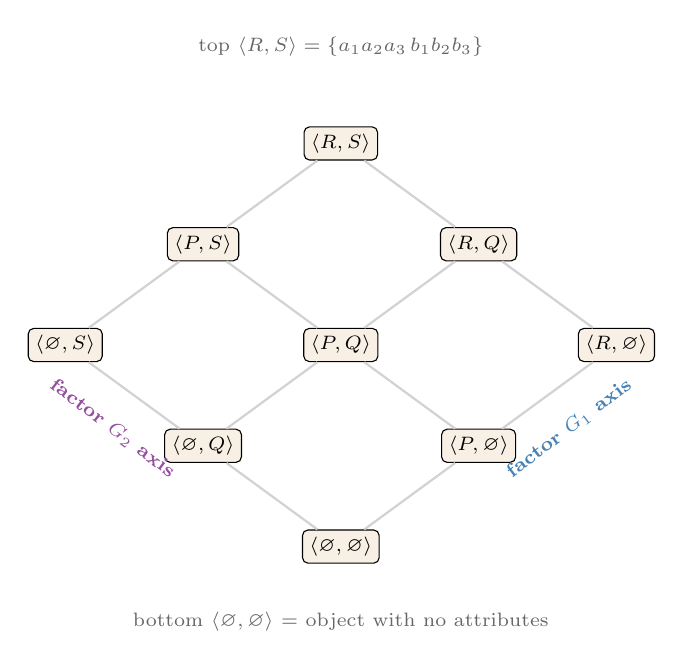
\begin{tikzpicture}[scale=1.0,
   gnode/.style={draw,rounded corners=2pt,fill=cConc!12,inner sep=2.5pt,font=\scriptsize},
   every edge/.style={draw,cGrid,thick}]
 % position: x' = (i - j)*1.7 , y' = (i + j)*1.25 ; i = factor-1 level, j = factor-2 level
 \foreach \i/\Pa in {0/{\varnothing},1/{P},2/{R}} {
   \foreach \j/\Pb in {0/{\varnothing},1/{Q},2/{S}} {
     \pgfmathsetmacro{\x}{(\i-\j)*1.75}
     \pgfmathsetmacro{\y}{(\i+\j)*1.28}
     \node[gnode] (n\i\j) at (\x,\y) {$\langle \Pa,\Pb\rangle$};
   }
 }
 % cover edges: up in factor 1 (i->i+1) and factor 2 (j->j+1)
 \foreach \i/\ii in {0/1,1/2}
   \foreach \j in {0,1,2}
     \draw (n\i\j) edge (n\ii\j);
 \foreach \j/\jj in {0/1,1/2}
   \foreach \i in {0,1,2}
     \draw (n\i\j) edge (n\i\jj);
 % axis annotations
 \node[text=cFacA,font=\scriptsize\bfseries,rotate=37] at (2.9,1.5) {factor $G_1$ axis};
 \node[text=cFacB,font=\scriptsize\bfseries,rotate=-37] at (-2.9,1.5) {factor $G_2$ axis};
 \node[font=\scriptsize,text=black!60,align=center] at (0,-0.95)
   {bottom $\langle\varnothing,\varnothing\rangle$ = object with no attributes};
 \node[font=\scriptsize,text=black!60,align=center] at (0,6.35)
   {top $\langle R,S\rangle=\{a_1a_2a_3\,b_1b_2b_3\}$};
\end{tikzpicture}
\caption{The lattice generated by the coproduct of Figure~\ref{fig:coproduct}: a
$3\times 3$ grid, i.e.\ the direct product of two $3$-chains. Each node is a
\emph{pair} $\langle$factor-1 state, factor-2 state$\rangle$; its attribute set is
the union of the two states' attributes. The DAG stores only the two \emph{axes}
(four concept nodes); the nine grid points are generated, never stored. Moving up
a north-east edge advances the $G_1$ coordinate, up a north-west edge the $G_2$
coordinate --- the hallmark of a product order.}
\label{fig:grid}
\end{figure}

% =======================================================================
\section{What the identity buys, and how it sits in known mathematics}
\label{sec:buys}
% =======================================================================

\begin{corollary}[Additive description, multiplicative expressiveness]
\label{cor:size}
$\bigl|\Lgen(G_1\Gcoprod G_2)\bigr| = |\Lgen(G_1)|\cdot|\Lgen(G_2)|$, while the
generator $G_1\Gcoprod G_2$ has $|G_1|+|G_2|$ nodes and edges. For $k$ pairwise
attribute-disjoint factors the represented lattice has $\prod_i|\Lgen(G_i)|$
concepts and the generator has $\sum_i|G_i|$ parts. With $k$ single-concept
binary factors this is $2^{k}$ concepts from $k$ generators.
\end{corollary}

This is the exponential gap between a factorial code and the concept lattice it
stands for, written as an identity rather than a slogan. The generator is a
\emph{compressed} presentation of the lattice; the compression ratio is exactly
the ratio of a sum to a product. Description-length-wise: the structure cost of
storing the coproduct is additive in the factors, whereas materialising the
product lattice as an explicit set of concepts is multiplicative --- which is why
any code that lands on the coproduct pays only the additive price. (This is a
statement about the \emph{structure} term alone; it holds for any monotone code
over the generators, and needs no assumption about the data.)

\paragraph{Where this meets classical FCA.} Two standard facts frame the result.
First, apposition: if the same objects are described by two disjoint attribute
blocks and one apposes the contexts, the concept lattice of the combined context
is a \emph{subdirect product} of the two block lattices --- it embeds in their
direct product via extent intersection, and \emph{equals} the full product
exactly when every combination of block-extents is realised by some
object~\cite{ganter1999}. Second, subdirect decomposition: by Birkhoff's theorem
every (finite) lattice is a subdirect product of subdirectly
irreducibles~\cite{birkhoff1944,davey2002}. So ``factor this concept lattice''
\emph{is} the subdirect-decomposition problem --- genuinely nontrivial to run
backwards on an already-built lattice.

Theorem~\ref{thm:main} sits on the \emph{generator} side of this picture and is
correspondingly clean. Two points are worth keeping distinct:
\begin{itemize}
  \item The lattice generated by the coproduct is the \emph{full} direct product
        $\Lgen(G_1)\times\Lgen(G_2)$, because the DAG can switch on any
        combination of factor states regardless of what any data set contains.
  \item The lattice \emph{realised by a particular data set} is the subdirect
        product of the classical result --- the full product intersected with
        ``which combinations actually occur.''
\end{itemize}
The gap between them is precisely which product cells are populated. A learner's
job is to install a coproduct generator whose full product \emph{covers} the
realised subdirect lattice, at additive cost --- and, crucially, to do so
\emph{without} ever materialising the product and running Birkhoff backwards.
Building the factors directly sidesteps the hard decomposition entirely.%
\footnote{A terminological caution: FCA also has a \emph{direct product of
contexts} (object set $G_1\times G_2$, a specific incidence) whose lattice is the
\emph{tensor} product, a different construction~\cite{ganter1999}. The operation
relevant here is \emph{apposition} of two attribute blocks over the \emph{same}
objects, whose lattice is a subdirect product of the direct product of the factor
lattices. Theorem~\ref{thm:main} is about the direct product of the
\emph{generated} lattices, on the generator side.}

% =======================================================================
\section{The neural-code reading}
\label{sec:neural}
% =======================================================================

FCA's foundational equivalence is that a formal context (objects $\times$
attributes) and its concept lattice are two views of one thing, convertible both
ways. A \emph{neural code} in Barlow's sense~\cite{barlow1961,barlow1989} is the
same data seen a third way: each object is a binary vector saying which
\emph{units} are active. In our model the units are the DAG's nodes, the code for
an object is the indicator of its activated antichain, and the decoder
$\Dcode_G$ is a fixed monotone Boolean map (an OR of closures) from code to
attributes. Theorem~\ref{thm:main} then reads, in code terms:

\begin{quote}
\emph{An additive architecture of units --- two groups with no cross-wiring ---
under OR-of-closures decoding represents the multiplicative (product) space of
concepts. Every combination of a factor-$1$ state and a factor-$2$ state is a
representable object, expressed by co-activating one unit-group from each factor,
\emph{not} by a dedicated ``combination'' unit.}
\end{quote}

This is exactly Barlow's \emph{factorial code}~\cite{barlow1989,barlow1972,
foldiak1990,foldiak1995,olshausen1996}: independent factors of variation get
independent groups of units; the combinatorial multitude of joint concepts is
carried by \emph{which units co-fire}, never by enumerating grandmother units for
each combination. The exponential compression a factorial/sparse code delivers is
the same fact as Corollary~\ref{cor:size}, now told about firing patterns instead
of lattice nodes.

\begin{figure}[h]
\centering
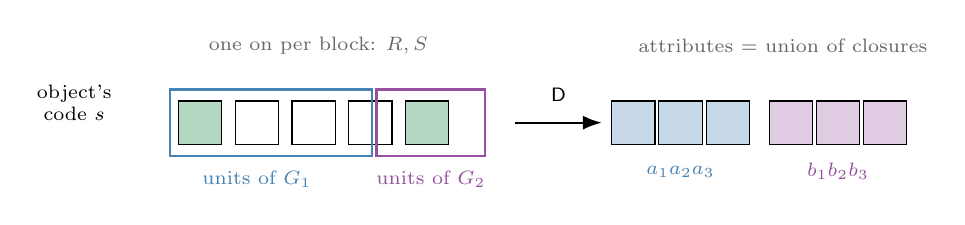
\begin{tikzpicture}[font=\footnotesize,
   unit/.style={draw,minimum size=5.5mm,inner sep=0pt},
   on/.style={fill=cGood!35}, off/.style={fill=white}]
 % code vector, two blocks
 \node[align=center,font=\scriptsize] at (-1.6,0.25) {object's\\code $s$};
 \foreach \i/\st in {0/on,1/off,2/off,3/off,4/on} {
   \pgfmathtruncatemacro{\lbl}{\i+1}
   \ifnum\i<3 \def\bc{cFacA}\else\def\bc{cFacB}\fi
   \node[unit,\st] (u\i) at (\i*0.72,0) {};
 }
 \draw[cFacA,thick] (-0.38,-0.42) rectangle (2.18,0.42);
 \draw[cFacB,thick] (2.24,-0.42) rectangle (3.62,0.42);
 \node[text=cFacA,font=\scriptsize] at (0.72,-0.72) {units of $G_1$};
 \node[text=cFacB,font=\scriptsize] at (2.93,-0.72) {units of $G_2$};
 \node[font=\scriptsize,text=black!60,align=center] at (1.5,0.98)
   {one on per block: $R,S$};
 % arrow
 \draw[-{Latex[length=2.4mm]},thick] (4.0,0) -- (5.1,0);
 \node[font=\scriptsize] at (4.55,0.35) {$\Dcode$};
 % decoded attributes
 \foreach \i/\st in {0/on,1/on,2/on} \node[unit,\st,fill=cFacA!30] (a\i) at (5.5+\i*0.6,0) {};
 \foreach \i/\st in {0/on,1/on,2/on} \node[unit,\st,fill=cFacB!30] (b\i) at (7.5+\i*0.6,0) {};
 \node[font=\scriptsize,text=cFacA] at (6.1,-0.62) {$a_1a_2a_3$};
 \node[font=\scriptsize,text=cFacB] at (8.1,-0.62) {$b_1b_2b_3$};
 \node[font=\scriptsize,text=black!60,align=center] at (7.4,0.98)
   {attributes = union of closures};
\end{tikzpicture}
\caption{The same fact as a code. The unit vector splits into two blocks with no
cross-wiring (additive architecture). Firing one unit per block and decoding by
union of closures yields one cell $\langle R,S\rangle$ of the product lattice of
Figure~\ref{fig:grid}. All $3\times 3$ cells are reachable this way; none needs a
dedicated ``$R$-and-$S$'' unit.}
\label{fig:code}
\end{figure}

\paragraph{``Learn the code'' vs.\ ``learn the DAG'' is not a dichotomy.}
A recurring temptation is to abandon the DAG and simply learn a sparse binary
code as most of machine learning does, mapping to a DAG later --- with the worry
that mapping a learned code \emph{to factored graphs} is itself hard. The model
here dissolves the choice: the DAG \emph{is} the decoder (the codebook) and the
per-object antichain \emph{is} the code; learning them is one act, not two. And
the factorisation one would otherwise have to recover by hand falls out for free,
because in a coproduct the factors are literally the \emph{connected components}
of the generator graph (Figure~\ref{fig:coproduct}). Reading a learned coproduct's
factors is a linear-time graph traversal; reading a materialised product's factors
is subdirect decomposition. The lesson is to keep the representation \emph{folded}
(a coproduct of small generators) rather than unfold it into a product and try to
refold --- the same conclusion Barlow's efficient-coding argument reaches from the
redundancy side.

% =======================================================================
\section{Boundary conditions worth remembering}
\label{sec:boundary}
% =======================================================================

The identity is clean but conditional. Three conditions matter, and it is worth
being explicit about which are needed for the \emph{representation} theorem and
which only for a \emph{learner} to prefer the factored form.

\paragraph{(B1) Disjoint alphabets --- needed for the theorem.} The whole proof
rests on $\attrs_1\cap\attrs_2=\varnothing$ so that intersection recovers the two
parts. If the two factors \emph{share} an attribute, that attribute cannot be
assigned to one part, $\varphi$ is no longer a bijection, and $\Lgen(G_1\Gcoprod
G_2)$ is only a \emph{subdirect} product --- the connected components no longer
cleanly separate. Attribute-level entanglement between factors is exactly the
``overlapping concepts'' regime studied in the companion note, and it is where the
product story stops being exact. So the product-lattice blow-up (independent
blocks) is, perhaps counterintuitively, the \emph{benign} case; the hard case is
overlap \emph{within} a block.

\paragraph{(B2) Statistical independence --- needed for a learner to \emph{prefer}
the coproduct.} The theorem says the coproduct \emph{can represent} the product;
it does not say a description-length learner will \emph{choose} the coproduct over
some partly-materialised product. That is a separate, data-dependent fact. Under
per-use (usage) pricing, a dedicated cross-factor concept for a combination
$\langle A,B\rangle$ earns coding bits only if that combination occurs
\emph{more often than independence predicts} --- i.e.\ only if the factors are
statistically dependent (positive pointwise mutual information). For independent
factors the cross concept has zero information gain and cannot pay its usage rent,
so the learner declines it and the coproduct is the optimum. For \emph{dependent}
factors, some cross concepts do pay, and the true optimum is a \emph{partial}
product --- a few combination nodes grafted onto the two factors. Keeping (B1) and
(B2) separate is important: (B1) is algebra, (B2) is statistics.

\paragraph{(B3) Realisability --- which product cells the data populates.} Even
with disjoint, independent factors, a finite sample may not exhibit every one of
the $|\Lgen(G_1)|\cdot|\Lgen(G_2)|$ combinations. The generator still
\emph{represents} them all (the theorem is about representability); the data
merely exercises a subset. This is the gap between the full product (generator
side) and the subdirect product (data side) of \S\ref{sec:buys}.

% =======================================================================
\section{Empirical confirmation}
\label{sec:experiment}
% =======================================================================

We checked the prediction directly with the project's MDL learner (whose scoring
is described in the companion note). We planted two \emph{independent} two-level
hierarchies on disjoint $15$-attribute blocks, concatenated them into one
$30$-attribute matrix over $N=1000$ objects, and --- to put the product-lattice
pressure at maximum --- arranged that \emph{all} $36$ combinations of an
$A$-concept and a $B$-concept co-occur in the data. Classical FCA on this matrix
would materialise (a large part of) the $6\times 6$ product. The learner sees only
the matrix.

\begin{table}[h]
\centering
\begin{tabular}{lc}
\toprule
quantity & value \\
\midrule
co-occurring $(A\text{-concept},B\text{-concept})$ pairs in data & $36/36$ (full product pressure) \\
concepts the learner returns & $10$ \\
\quad of which \textbf{cross-block} (attributes in both blocks) & $\mathbf{0}$ \\
learned concepts confined to block $A$ / block $B$ & $5$ / $5$ \\
objects whose code activates a concept from \emph{both} factors & $991/1000$ \\
worst per-factor planted-concept extent Jaccard & $0.79$ (A), $0.78$ (B) \\
\bottomrule
\end{tabular}
\caption{Two independent planted factors, concatenated, handed to the MDL learner.
It returns the two factors as \emph{disconnected components} (five concepts each,
zero cross-block), and represents the product in the object codes: almost every
object co-activates one concept from each factor. The worst-case factor recovery
($0.79$) sits just under the project's $0.80$ match threshold --- a small-block,
finite-noise artefact --- but the \emph{structural} claim, zero cross-block
concepts, is exact. This is Theorem~\ref{thm:main} in the direction (B2) predicts:
independent factors $\Rightarrow$ coproduct optimum.}
\label{tab:experiment}
\end{table}

The learned loading graph is literally two connected components, one per block;
the product lives entirely in the antichain codes (Figure~\ref{fig:code}), never
in the concept set. That is the theorem and the boundary condition (B2) behaving
exactly as claimed. The experiment script is preserved with this note (see the
project README) for re-running.

% =======================================================================
\section{Relation to the project, and open directions}
\label{sec:project}
% =======================================================================

Within the \texttt{mdl-fca} project this note answers a design worry: that
learning ``one DAG'' would force the exponential product lattice into a single
tangled graph. It does not. With disjoint, independent feature groups the
description-length optimum is the coproduct of the per-group DAGs, and the product
is carried by the codes --- so the ideal ``product of factor DAGs'' is what the
learner already produces, as an emergent disconnected graph, with no factorisation
penalty and no mutual-information term added by hand. But the note is written to
stand alone: the core (Lemma~\ref{lem:separable}, Theorem~\ref{thm:main}) is a
fact about separable closure codes and factorial representations, true of any
learner or none.

Directions worth pursuing later:
\begin{itemize}
  \item \textbf{Make the factorisation a first-class output.} The learner returns
        one (disconnected) DAG; emitting its connected components as named factors
        is a linear-time post-step (\S\ref{sec:neural}). Worth doing so the model
        \emph{reports} ``this is $G_1\Gcoprod G_2$'' rather than leaving it
        implicit in the connectivity.
  \item \textbf{Partial products for dependent factors (B2).} When factors are not
        independent, characterise which cross concepts pay rent, and whether the
        learner recovers the minimal set of ``bridge'' concepts --- the graded
        interpolation between full coproduct and full product.
  \item \textbf{Interaction with overlap (B1).} The companion note's
        overlapping-concept limitation and this note's disjoint-alphabet condition
        are the same boundary seen from two sides. A usage code that lets a shared
        child pay rent (conditional/DAG-aware coding, or noisy-OR) is also what
        would let entangled factors be represented; unifying the two is the natural
        next theoretical step.
  \item \textbf{Beyond closure decoders.} Lemma~\ref{lem:separable} needs only
        separability, not closure. Any decoder that writes disjoint output blocks
        from disjoint unit blocks factors the same way; mapping which richer
        decoders (noisy-OR, thresholded linear) still yield clean products would
        extend the result past deterministic closure.
\end{itemize}

% =======================================================================
\section*{Summary}
% =======================================================================
\addcontentsline{toc}{section}{Summary}

An additive combination of concept generators represents a multiplicative concept
lattice. Precisely: over disjoint attribute alphabets, the coproduct of two
closure DAGs generates the direct product of the lattices they generate
individually (Theorem~\ref{thm:main}), because closure decoding is a separable
decoder and separable decoders factor (Lemma~\ref{lem:separable}). The generator
grows as a sum while the represented lattice grows as a product --- the exponential
compression of a factorial code, stated as a lattice identity
(Corollary~\ref{cor:size}) rather than an intuition. Read as a neural code, this
says independent factors of variation deserve independent, non-interacting groups
of units, with every joint concept carried by co-activation rather than a
dedicated unit --- Barlow's factorial code --- and it dissolves the apparent choice
between learning a sparse code and learning a DAG, since the DAG is the decoder,
the code is the activation, and the factorisation is just the generator's
connected components. The identity is exact under three conditions worth
remembering: disjoint alphabets (algebra, needed for the theorem), statistical
independence (statistics, needed for a compressor to \emph{prefer} the factored
form), and realisability (which product cells the data populates). A direct
experiment confirms it: a description-length learner given two independent planted
hierarchies returns the two factors and zero cross-factor concepts, representing
all their combinations in the object codes.

\bibliographystyle{plain}
\bibliography{refs}

\end{document}
